\chapter{Bidirectional current measurement}\label{ch:bidircurrent}
%**********************************************
\section{Overview}
In figure \ref{fig:block} the highlighted blocks were added into the previous structure, the blocks highlighted in red are covered in this report. The current sense circuitry was added at its position after the load so that the current it will measure is the current discharging from the battery or charging into the battery. The current sense amplifier will be used to produce a voltage between 0V and 5V that will correspond proportionally to the current in a designed range of 3V. The load can also be connected and disconnected with the help of the designed low side switch.


\begin{figure}[!htb]
\centering
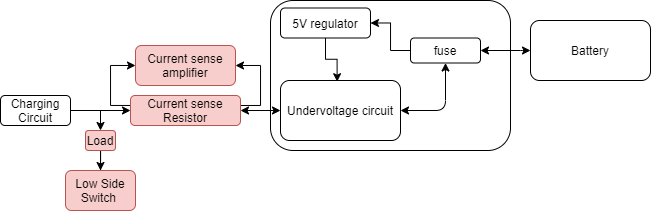
\includegraphics[scale=0.5]{./Figures/block}
\caption{Block Diagram showing circuit structure}
\label{fig:block}
\end{figure}

\subsection{Literature}
The bidirectional current sense amplifier is an op amp that is setup internally as can be seen in figure \ref{fig:data}. This internal circuitry is necessary because the resistors used need to be very accurate in order for current sensing to be accurate \cite{utube}. Another reason that the tsc213 is being used over a conventional op amp is because this device has a absolute differential voltage of 26V and a common mode voltage range of $gnd-0.3V$ to 26V. This is important for us because we can have differential voltages of up to 7.2V ($7.2-0$) and common mode voltages of about 7.2V which would not work with the previously used MCP op amp. The current sense amplifier will have its positive and negative inputs connected across a shunt resistor, the current sense amplifier will then amplify this difference by 50 (refer to \ref{fig:data}).


\subsection{Design}
When designing the current sense amplifier the current range that will be used should be considered. The most current that should be discharged from the battery should be 100mA. The maximum that the battery should charge at is 400mA. The current range was then determined to be $-150mA<I_{range}<450mA$, the additional 50mA was added as a safety factor to ensure the tsc213 does not breach the 0-5V output range. The output voltage range will be dependant on the differential voltage of the op amp and the reference voltage chosen (refer to eq \ref{eq:refeq}). The differential voltage will be dependant on the shunt resistance and the current through the shunt.
\begin{equation}
    V_o=(R_{shunt}\times I_{shunt})\times50+V_{REF}
    \label{eq:refeq}
\end{equation}
Using eq.\ref{eq:refeq} $R_{shunt}$ is designed to give an output voltage swing of 3V.
\begin{center}
    $V_{swing}=((R_{shunt}\times 0.45)-(R_{shunt}\times -0.15))\times 50$. \ \ $R_{shunt}=0.1$\textohm 
\end{center}
This results in voltage range across the shunt of $-15mV<V_{shunt}<45mV$. With a 0V at $V_{ref}$ the output range (using eq.\ref{eq:refeq}) would be -0.75V to 2.25V. This is not within 0V to 5V, this is where $V_{ref}$ is used to place the output voltage into a desirable range. The minimum $V_{ref}$ to get the output into the desired range would be 0.75V. The maximum $V_{ref}$ that would place the maximum output voltage at 5V would be 2.75V (i.e. 5-2.25). The average of the maximum and minimum $V_{ref}$ is then taken and found to be 1.75V. By doing this output voltage will be equally far from the upper and lower bounds of the 0V to 5V specification. To achieve this 1.75V the voltage from a 5V regulator is divided with resistors (refer to figure \ref{fig:circ}). \newline

To reduce the noise at the output a low pass filter was designed and placed at the output of the TSC213. 
\begin{equation}
    f_c=\frac{1}{2\pi RC}
    \label{eq:f}
\end{equation}
Using equation \ref{eq:f} and designing for 50Hz cutoff with a chosen resistor of 1.5k\textohm  \cite{lowpass}. For the chosen resistance a capacitance of 2.2\textmicro F was calculated. The reason 50Hz is designed for is because that is the frequency of noise that the 12V wall plug introduces into the circuit. 

\begin{figure}[!htb]
\centering
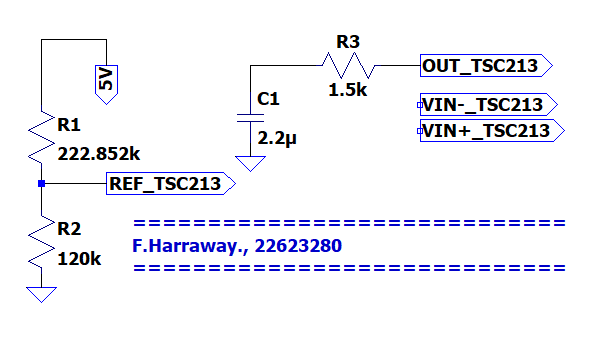
\includegraphics[scale=0.45]{./Figures/circ.png}
\caption{Oscilloscope Measurements}
\label{fig:circ}
\end{figure}

\newpage
\section{Results}

 \begin{figure}[!htb]
 \footnotesize
 \centering
    \begin{subfigure}[]{0.48\textwidth}
              \centering
  		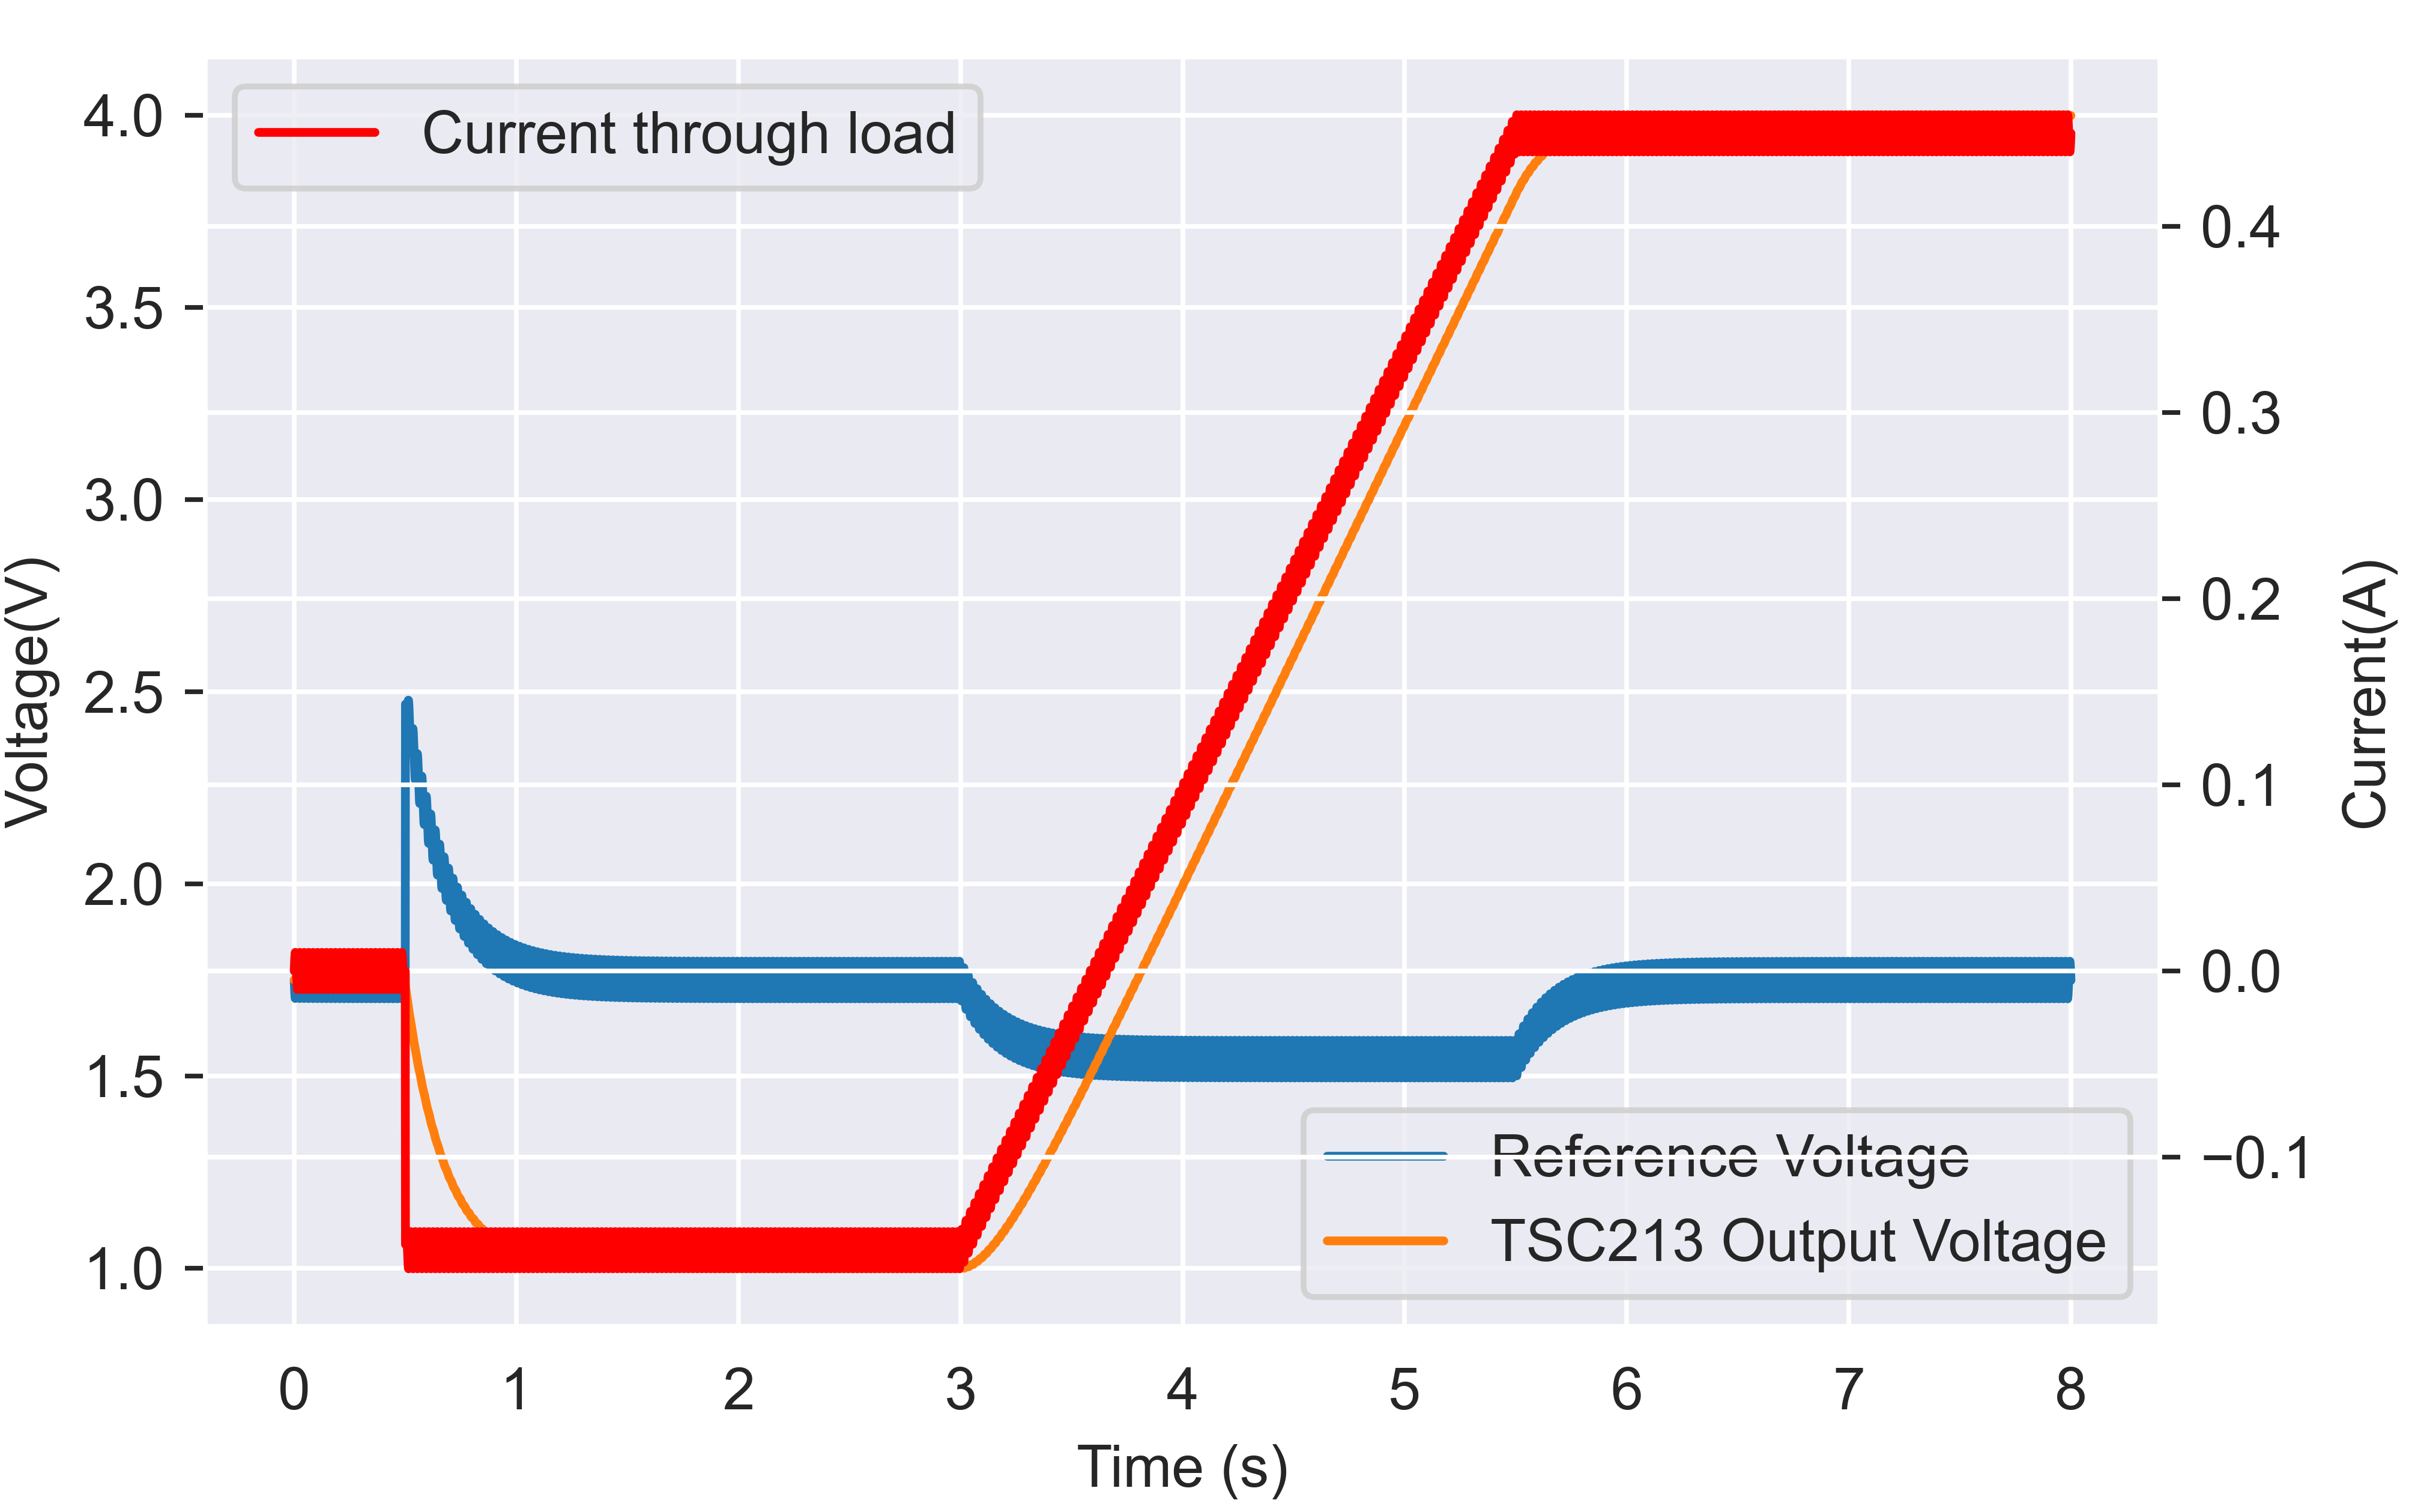
\includegraphics[width=1\linewidth]{./Figures/circuit.png}
		    \caption{} \label{subfig:sim}
     \end{subfigure}
     \begin{subfigure}[]{0.5\textwidth}
             \centering
  		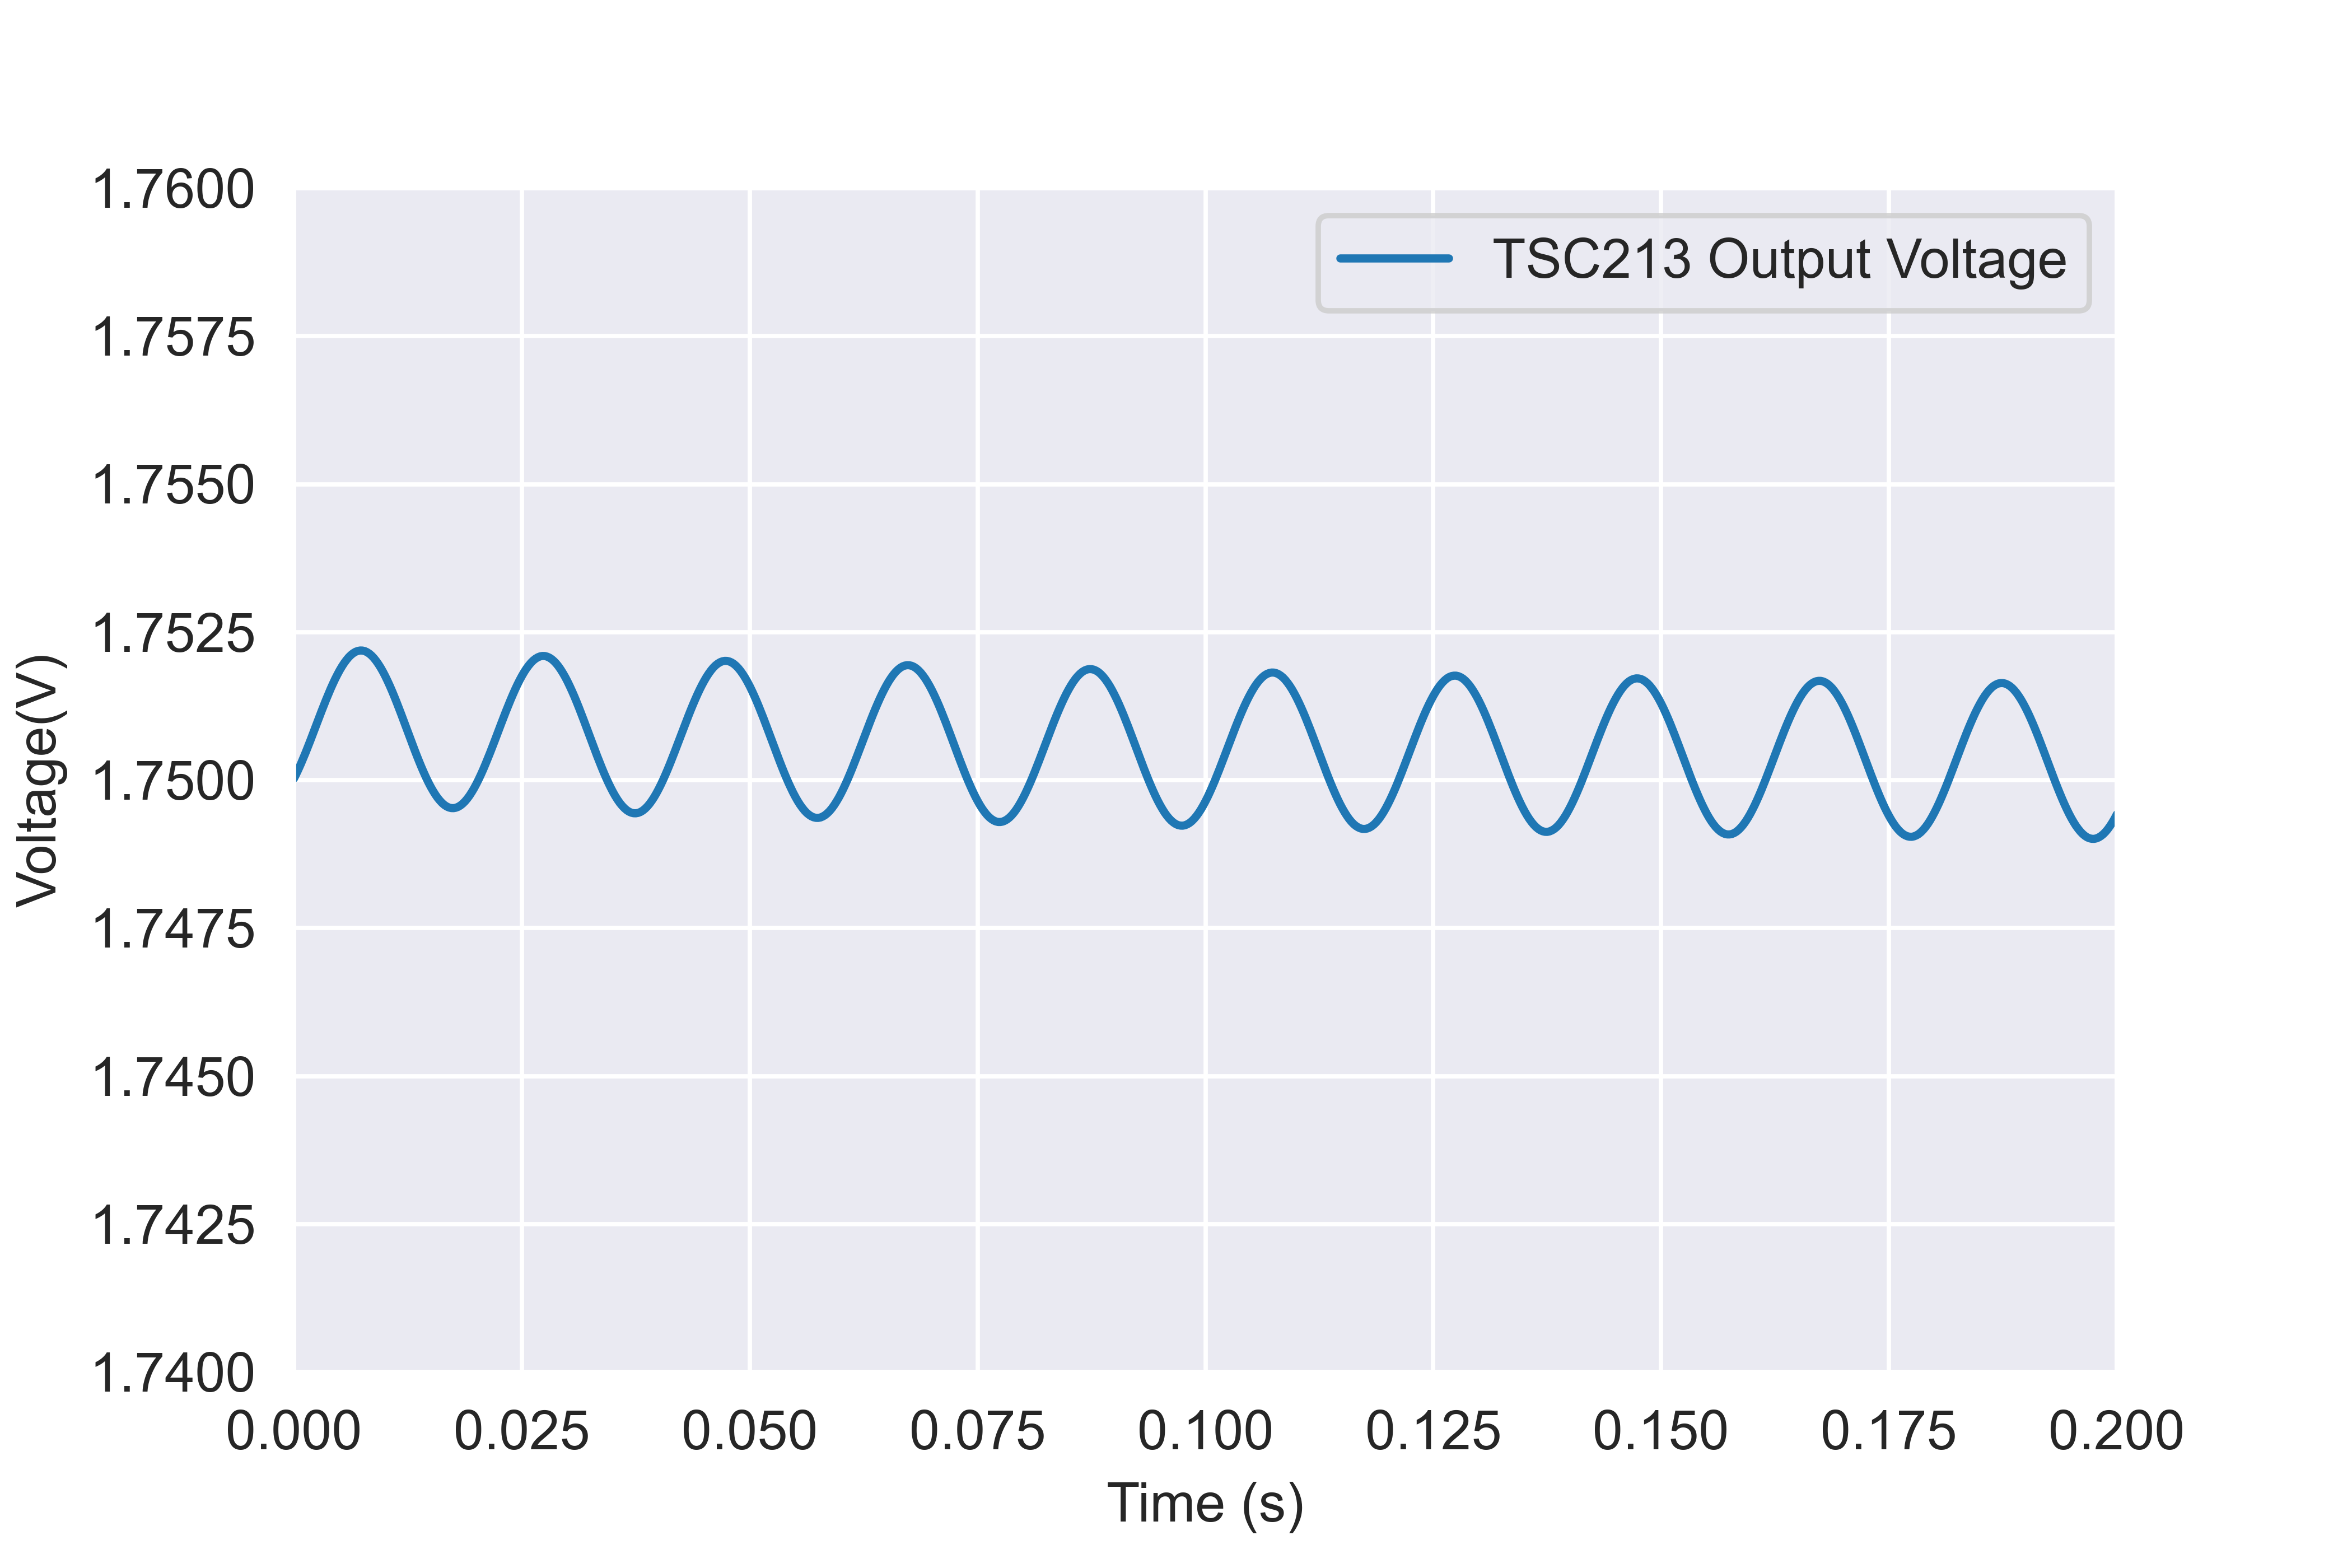
\includegraphics[width=1\linewidth]{./Figures/noise.png}
		   \caption{ } \label{subfig:noise}
     \end{subfigure}
   \caption[{Spice}]{LT Spice results   (a)  Simulation results (b)Noise in output signal }
 
 \end{figure}


\begin{figure}[!htb]
\centering
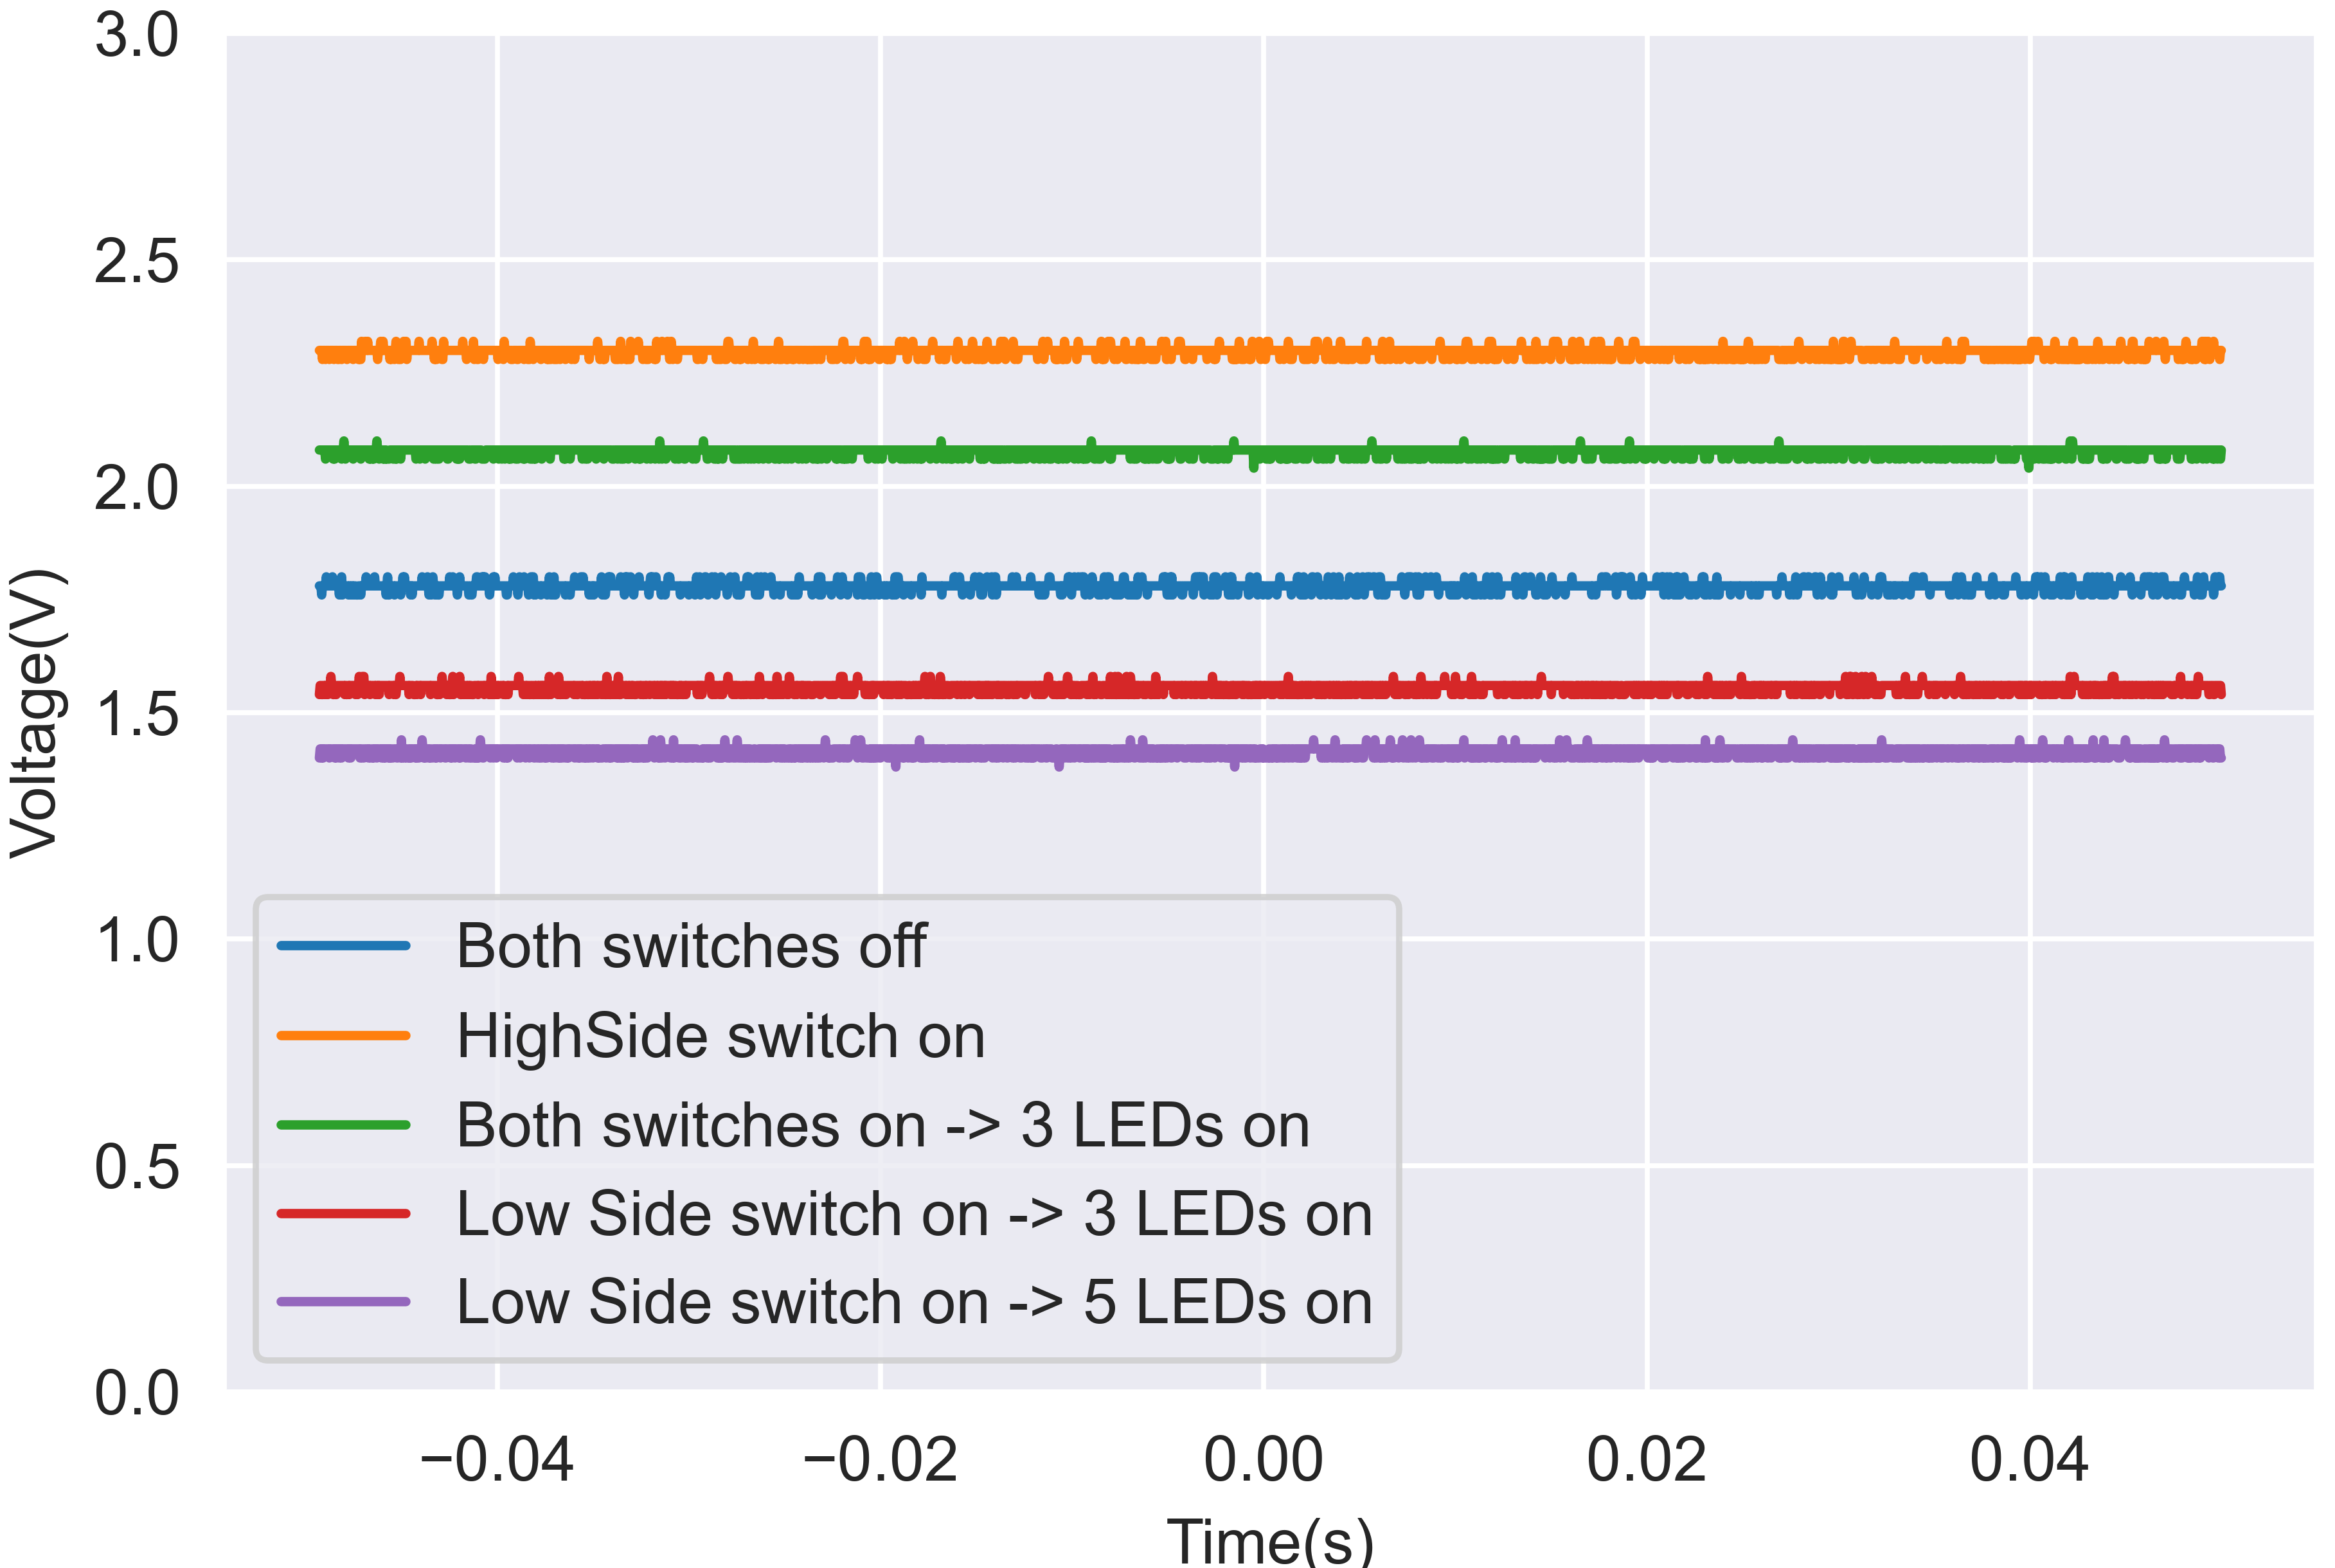
\includegraphics[scale=0.7]{./Figures/meas.png}
\caption{Oscilloscope Measurements}
\label{fig:meas}
\end{figure}

\begin{table}[!htb]
        \centering
        \footnotesize
        \caption{Resistor measurements}
         \begin{tabular}{lrrrr}
          \toprule
             & $Resistor \ Voltage$ & $Calculated \ Current$ \\
             &  [V]  & [mA]\\
          \midrule
         R1      & 3.35 & 15.23 \\
          R2 & 3.34   & 15.18 \\
          R3       &3.36 & 15.27 \\
          R4        &3.35 & 15.23 \\
          R4        &3.37 &15.32 \\
          \bottomrule
        \end{tabular}
     \label{tab:PVresults}
\end{table}
The LT spice simulations(figure \ref{subfig:sim}) show the output working correctly and the noise( figure \ref{subfig:noise}) is within spec. The measured noise on the output of the TSC213 was found to be 40mV ($V_{PK-PK}$) on the oscilloscope, however in the past I have found that oscilloscopes are not particularly accurate for these types of measurements. The general oscilloscope results are promising ( figure \ref{fig:meas}). The current through the LEDs is slightly less than 20mA as can be seen in table \ref{tab:PVresults}.
\vfill


